%!TEX root = ../paper.tex

The difference in results between the Modified Breiman Estimator and its shape adaptive variant on dataset \ferdosiOne, \baakmanOne, \baakmanFour, \baakmanFive raise several questions. This section attempts to answer them.

% Why are the estimations on Ferdosi 1 by SAMBE so much higher than those by MBE?
In \cref{fig:4:results:singleSphere} we observed that \sambe overestimates the densities of dataset \ferdosiOne. This could indicate that the kernels are too small, resulting in a too high contribution to the density estimate. Since the Modified Breiman estimator uses the same general and local bandwidth as the shape adaptive version the likely culprit is the shape of the kernel. This is confirmed by \cref{fig:discussion:baakman1:eigenVectors} which shows the eigenvectors of some of the used bandwidth matrices used. This figure clearly shows that the second and third eigenvectors are parallel , and all point to the right indicating that the kernels are overly elongated along the horizontal axis. 

\begin{figure}
	\centering
	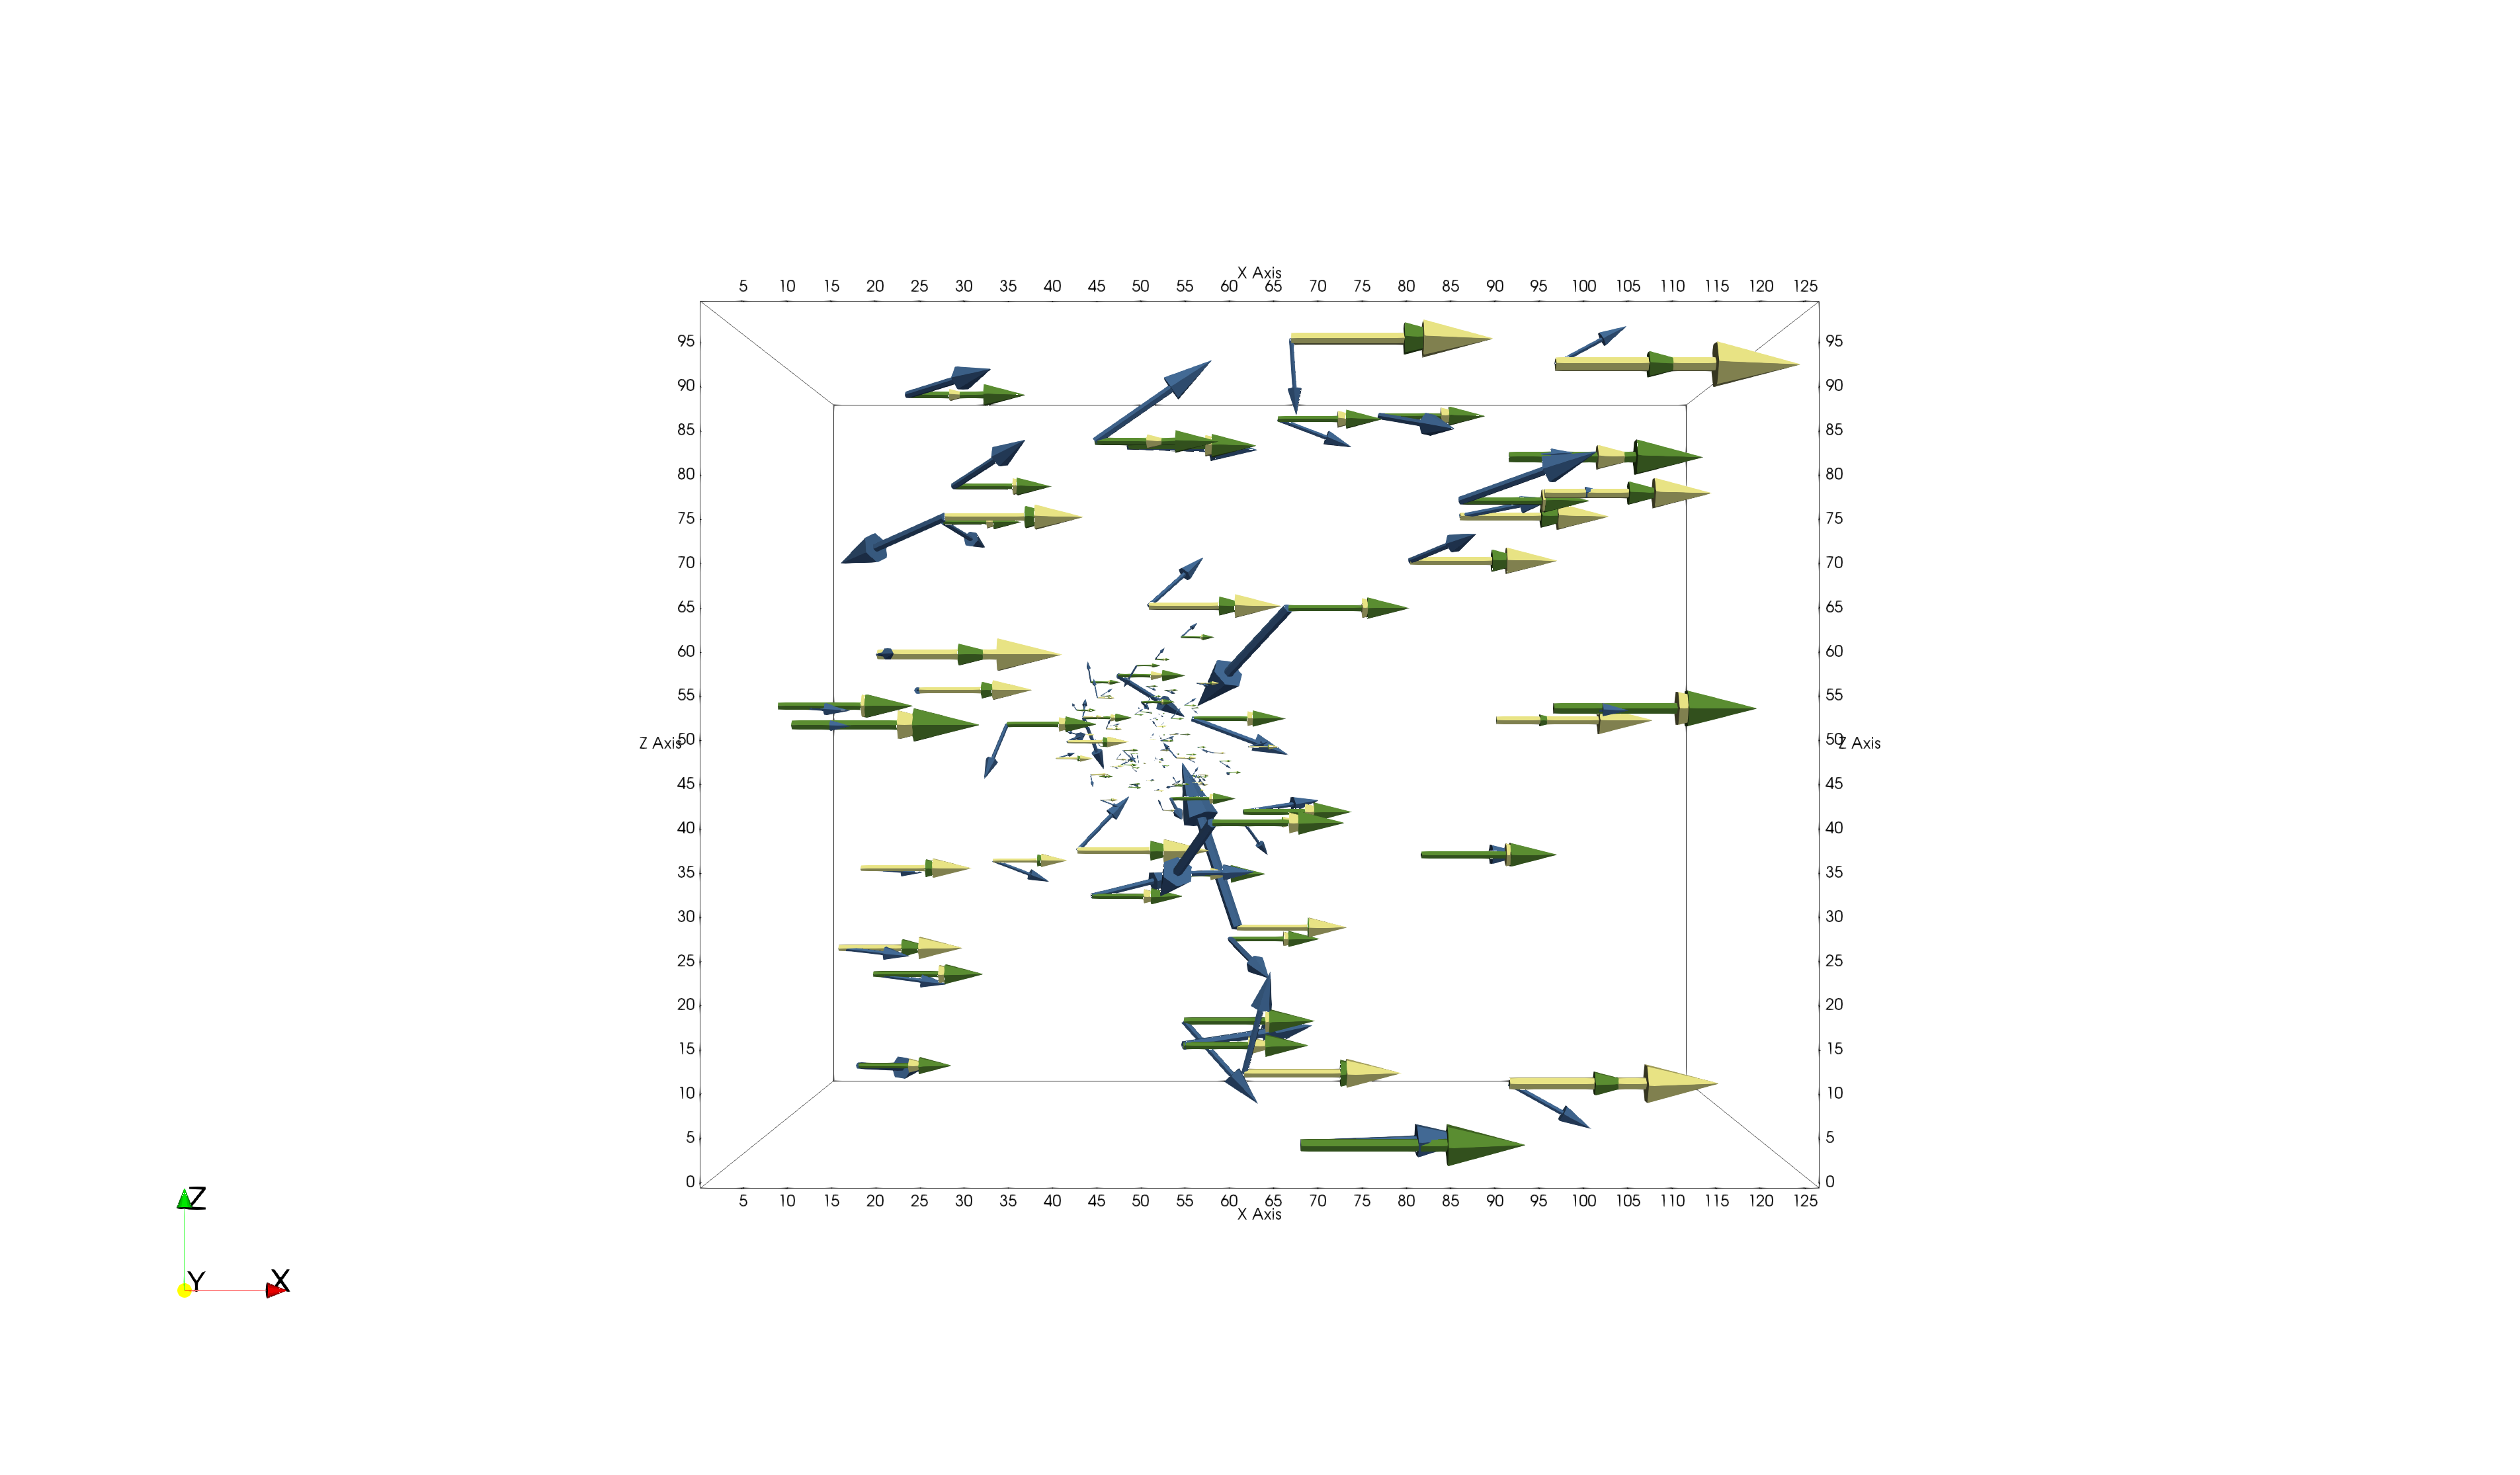
\includegraphics[width=\columnwidth, trim={950px 390px 950px 390px},clip]{5/img/baakman_1/baakman_1_eigen_vectors.png}
	\caption{The eigenvectors scaled by the associated eigenvalue of the bandwidth matrix of 120 spaced samples of dataset \baakmanOne. The first eigenvector of each pattern is shown in blue, the second in green and the third in yellow.}
	\label{fig:discussion:baakman1:eigenVectors}
\end{figure}

\todo[inline]{Why are some estimated densities smaller than zero with SAMBE on Baakman1, Baakman4, Baakman5?}
\todo[inline]{Why are some estimated densities greater than one with SAMBE on Baakman1, Baakman4, Baakman5?}
\todo[inline]{Why are the differences between baakman1, baakman4, baakman5 largest?, why not in ferdosi1?}